\documentclass[a4paper,10pt,headlines=3.2]{scrartcl}
\usepackage{graphicx}           %Bilder

%\usepackage[T1]{fontenc}        %Umlaute
%\usepackage[latin1]{inputenc}   %Windows
%\usepackage[utf8x]{inputenc}	%Linux
\usepackage{ucs}

\usepackage[ngerman]{babel}     %Deutsche Sprache
\usepackage{amsmath}            %Math. Zeichen
\usepackage{pifont}             %Skalierbare Schriftart
\usepackage{array}
\usepackage{epsfig}             %Erweiterte Grafiken
\usepackage{makeidx}            %Stichwortverzeichnis
\usepackage[pdftex]{color} 

\newcommand{\changefont}[3]{
\fontfamily{#1} \fontseries{#2} \fontshape{#3} \selectfont}

\makeindex

\usepackage[automark]{scrpage2}
\usepackage[nosectionbib]{apacite}               %Zitieren

%\usepackage[colorlinks]{hyperref}%Hyperlinks

\usepackage{lmodern}
\usepackage{scrpage2}           %KOMA-Script
\usepackage{tipa}
\usepackage{qtree}
\usepackage{pgf}


\usepackage{remreset}			%Fussnoten global
\makeatletter
\@removefromreset{footnote}{chapter}
\makeatother 

\setcounter{tocdepth}{3}

%Kopfzeilen
\pagestyle{scrheadings}         %Seitenstil scrheadings verwenden

%\setlength{\textheight}{24cm}
%\setlength{\textwidth}{16cm}
%\setlength{\topmargin}{-2cm}
%\setlength{\oddsidemargin}{0cm}

% Groesse des Textbereiches in der Seite
\setlength{\textwidth}{16cm}
\setlength{\textheight}{22cm}
% Kopf- und Fusszeile, Hoehe und Abstand vom Text
\setlength{\headheight}{15pt}
\setlength{\headsep}{0.8cm}
% Linker Seiteneinzug
\setlength{\oddsidemargin}{2.5cm} \addtolength{\oddsidemargin}{-1in}
\setlength{\evensidemargin}{2.5cm} \addtolength{\evensidemargin}{-1in}
% Andere Groessen ausrechnen (vertikal zentrieren)
\setlength{\footskip}{\headsep}
\addtolength{\footskip}{\headheight}
\setlength{\topmargin}{\paperheight}
\addtolength{\topmargin}{-\textheight}
\addtolength{\topmargin}{-\headheight}
\addtolength{\topmargin}{-\headsep}
\addtolength{\topmargin}{-\footskip}
\addtolength{\topmargin}{-2in}
\addtolength{\topmargin}{-0.5\topmargin}

%Schriftart
\changefont{cmss}{m}{n}

%Abstand zur�cksetzen
\setlength{\headheight}{20pt}

\usepackage{listings} 
\lstset{numbers=left, numberstyle=\tiny, numbersep=5pt} \lstset{language=Java} 

\clearscrheadfoot
%\renewcommand{\headheight}{40pt} 
\ihead[]{Datenstrukturen und Algorithmen \\Fr�hlingssemester 2011 \\Institut f�r angewandte Mathematik} % - links
\ohead[asdasd]{�bung 8 \\Abgabetermin 21. April 2011 \\Adrianus Kleemans [07-111-693]} % - linke Kopfzeile 
\setheadsepline{.4pt} %Separate Linie im Kopf
\cfoot[\pagemark]{\pagemark} %- mittlere Fusszeile 

\begin{document}
\section*{Theoretische Aufgaben: Rot-Schwarz-B�ume}
\subsection*{Aufgabe 1}
Da die Wurzel vorher rot war, m�ssen die beiden Unterknoten (falls vorhanden) schwarz sein. Die Eigenschaft 4 w�rde deshalb bei einer Schwarzf�rbung nicht verletzt werden, weshalb der resultierende Baum ein g�ltiger Rot-Schwarz-Baum sein muss.

\subsection*{Aufgabe 2}
Da jeder Pfad von einem Knoten zu seinem Blattknoten gleichviele schwarze Knoten haben muss, kann nur die Anzahl roter Knoten variieren. Beim k�rzesten Pfad entspricht dies nur schwarzen Knoten, beim l�ngsten gibt es gleichviele beider Farben. Da es h�chstens gleichviel schwarze wie rote Knoten geben kann, ist auch die L�nge des l�ngsten Pfads h�chstens doppelt.

\subsection*{Aufgabe 3}
\begin{itemize}
 \item \textbf{Minimale Anzahl:} Vom Buch: $2^{h}-1$ innere Knoten sind das Minimum.
 \item \textbf{Maximale Anzahl:} Bei maximaler Knotenanzahl muss jeder Pfad die maximale L�nge (2 $\cdot$ Schwarzh�he) haben. Daraus ergibt sich eine Knotenanzahl von $2^{2\cdot h}-1$.
\end{itemize}

\subsection*{Aufgabe 4}
\lstset{frame=single}
\begin{lstlisting}[caption=Aufgabe 4]{Name}
right-rotate(T, x)
y = x.links           // bestimme y
x.links = y.rechts     // mache y's rechter Teilbaum zu x's linkem

if y.rechts != T.nil    
  y.rechts.vater = x
y.vater = x.vater      // setze y's Vater auf x's Vater
if x.vater == T.nil
  T.wurzel = y
else if x == x.vater.rechts
  x.vater.rechts = y
else x.vater.links = y
y.rechts = x            // mache x zu y's rechtem Kind
x.vater = y
\end{lstlisting}

\subsection*{Aufgabe 5}
\begin{itemize}
 \item F�r jedes linke Kind kann die Operation right-rotate ausgef�hrt werden, solange, bis alle in den rechten �usseren Pfad (der Pfad, in dem alle Knoten ausser der Wurzel rechte Kinder sind) integriert wurden. Dies muss nicht f�r die Wurzel geschehen, deshalb reichen $n-1$ Rechtsrotationen.
 \item Wenn man vom degenerierten Baum, der nur aus einem rechten Pfad (wie oben beschrieben) besteht, die Rechtsrotationen mit Linksrotationen wieder r�ckg�ngig macht, so erh�lt man wieder den urspr�nglichen Baum. Da nun jeder Baum in die degenerierte Form umwandelbar ist, gilt auch das umgekehrte, aus dem degenerierten baum l�sst sich in $n-1$ Linksrotationen jeder gew�nschte Baum bauen. Die Gesamtlaufzeit ist deshalb $2\cdot(n - 1) = 2n -2$, welches in $\Theta(n)$ liegt.
\end{itemize}


\subsection*{Aufgabe 6}
Es werden gem�ss der Problemstellung nur Rot-Schwarz-B�ume gezeichnet und keine tempor�r erstellten Zwischenb�ume.
\begin{figure}[!ht]
\centering
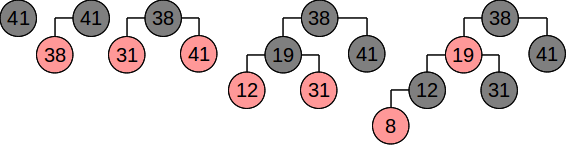
\includegraphics[width=.95\linewidth]{aufg6}
\end{figure}

\subsection*{Aufgabe 7}
Da die Wurzeln der Teilb�ume auch schwarz sind, kommt bei den unteren Knoten als Schwarzh�he zu $k$ schon eins dazu. 
\begin{figure}[ht]
\centering
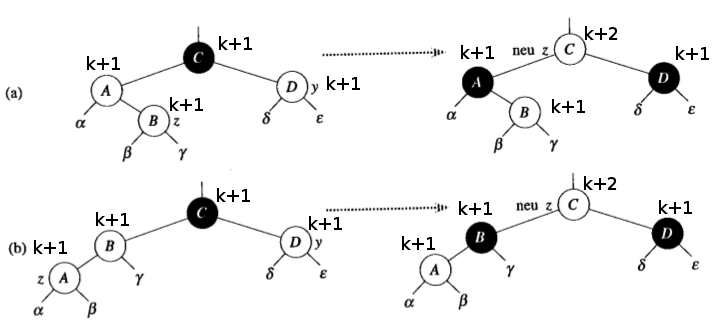
\includegraphics[height=5.6cm]{aufg7_1}
\end{figure}
\begin{figure}[ht]
\centering
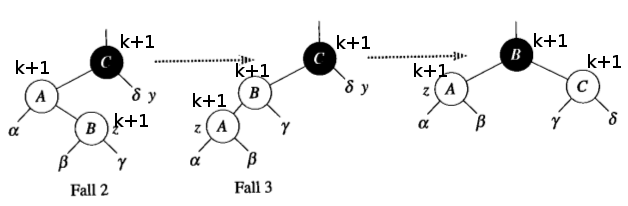
\includegraphics[height=4cm]{aufg7_2}
\end{figure}
Die Transformation erh�lt die Eigenschaft 5. �ber dem Knoten C oder allgemein dem angezeigten Teilbaum ist die H�he konstant k+2 geblieben.

\subsection*{Aufgabe 8}
Nein, durch die verschiedenen F�lle kann es zu Umformungen oder zu Umf�rbungen kommen. Der resultierende Baum muss nicht derselbe sein; ein right- oder left-rotate verformt ihn oder das Herstellen der Eigenschaft 4 kann einzelne Knoten verf�rben.

\end{document}